\section{Processor Optimizations}
\label{sec:processor_opt}

Our processor optimizations are based on the observation that arithmetic operations, such as addition and multiplication, which are a critical portion of training kernels have predetermined results if one of the input operands is a zero. We refer to instructions that perform such arithmetic operations as ``zero-optimizable'' instructions. Exploiting zero-optimizable instructions to improve training peformance is promising because our profiling studies show that a significant portion of computation involves zeroes. 

\begin{figure*}
\centering
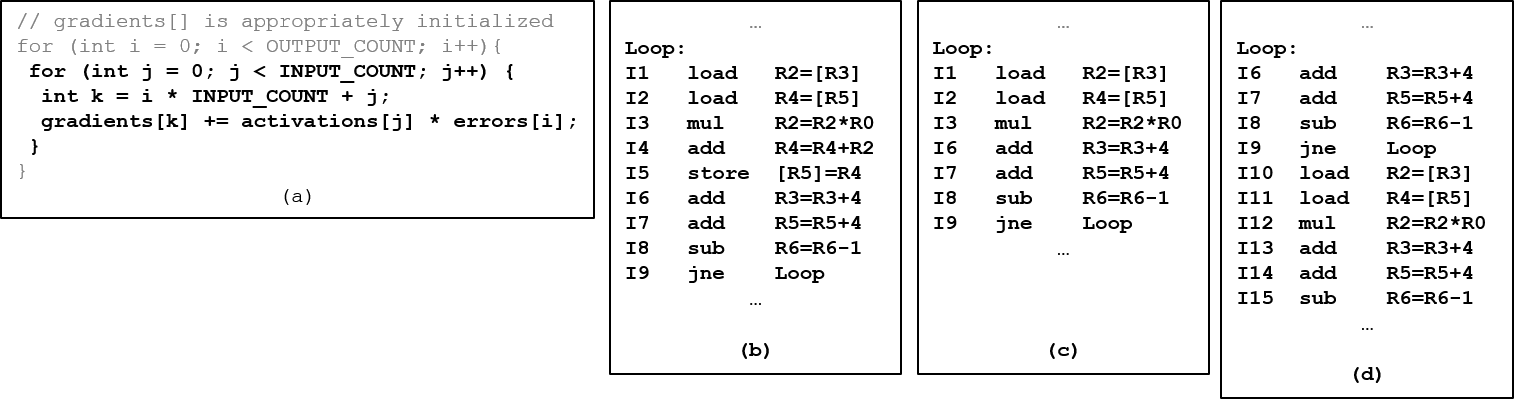
\includegraphics[width=1.9\columnwidth]{Figures/gradient_code_opt.png}
\caption{(a) Source code for computing gradients, (b) machine code of inner loop, (c) optimized code after basic instruction quashing, and (d) optimized code after advanced instruction quashing.}
\label{fig:gradient_code_opt}
\end{figure*}

\subsection{Opportunities}

In modern out-of-order processors, a zero-optimizable instruction in the instruction queue presents a number of optimization opportunties because its results and side effects are immediately known (without issuing to an execution unit) once an input operand resolves to zero.  As a result, the other data dependencies and some pipeline stages could become redundant in executing the instruction. This makes it possible to reduce execution cycles and pressure on processor resources by issuing or commiting zero-optimizable (and dependent) instructions earlier than normal or squashing them, as discussed below. 

\subsubsection{Training Code Example.}
We use the training code snippets presented in Figure~\ref{fig:gradient_code_opt} to describe our optimizations.  Figure~\ref{fig:gradient_code_opt}(a) illustrates simplifed code for computing gradients to update layer weights during back-propagation. Gradients are computed as an inner product of the activation and error vectors. From Figure~\ref{fig:cifar-10_word_sparsity}, a promising optimization is to skip multiply and addition operations if \emph{activations[j]} or \emph{errors[i]} is zero. Moreover, if \emph{errors[i]} is zero then the inner loop execution can skipped. While these optimizations could be achieved with software modifications, we realize similar optimizations dynamically with processor techniques based on zero-optimizable instructions.  We compare the software and hardware optimization approaches in our evaluation. {\color{red} Need stronger justification for why hardware optimization is necessary besides supporting existing binaries?}.

We use the machine code sequences in Figures~\ref{fig:gradient_code_opt}(b), ~\ref{fig:gradient_code_opt}(c), and ~\ref{fig:gradient_code_opt}(d), which correspond to the inner loop, to illustrate the impact of our optimizations on instructions in the instruction queue.  Although there are six zero-optimizable instructions in the loop (I$3$, I$4$, I$6$, I$7$, and I$8$), the optimizations discussed invole only I$3$ and I$4$. We assume that R$0$, which corresponds to \emph{errors[i]}, is zero. 

\subsubsection{Early Instruction Issue/Commit.}  First, a zero-optimizable instruction can be issued once the zero operand is available if it makes other operands redundant.  For example, I$3$ can be issued early becaue it is a multiplication and the zero value of R$0$ makes R$2$ redundant.  Second, a zero-optimizable instruction could be committed early if the zero input determines its results and side effects. This is also the case for I$3$. Early issue and commit of zero-optimizable instructions can reduce pressure on processor resources and wait times of data dependent instructions, such as I$4$, since the dependencies are satisfied sooner. 

\subsubsection{Instruction Squashing.} A zero-optimizable instruction can be squashed in the instruction queue if a zero input operand makes it an identity function and thus redundant. For this reason, I$4$ can be squashed since it is an addition and R$2$ is zero. Squashing an instruction can make the  instructions that it depends on (producers) and those that depend on it (consumers) redundant, leading to more instruction squashing.  For example, I$5$ becomes redundant (a silent store) and can be squashed, if I$5$ is squashed. Figure~\ref{fig:gradient_code_opt}(c) shows the impact of squashing I$4$ and I$5$.  We further observe that  I$1$, I$2$, and I$3$ are now redundant in all but the last loop iteration, since their results (R$2$ and R$4$) are not used.  We can squash these three instructions in all but the last iteration as shown in Figure~\ref{fig:gradient_code_opt}(d). Compared to the orignal machine code sequence, the optimized code sequence will run much faster because of the squashed instructions, especially loads which often have high latency.  Thus, by exploiting zero-optimizable instructions we can improve the performance of the inner loop of the gradient computation code. 

\subsection{Mechanisms}
Our optimizations can be realized with minor extensions to the front-end processing of a modern out-of-order processor. The extensions are lightweight, and despite being on the critical path should not introduce noticeable execution delays. Specifically, we propose processor extensions to do the following operations: (i) identify zero-optimizable instructions, (ii) detect when zero-optimizable input operand is a zero, (iii) modify producer and consumer data dependencies, and (iv) squash instructions.  These steps can be done in parallel with existing pipeline front-end stages, as we discuss below. 

\subsubsection{Identify Zero-Optimizable Instructions.} We can detect zero-optimizable instructions during instruction decoding by matching the opcode against a predefined set of opcodes. Since only a small set of arithmetic instructions qualify as zero-optimizable, the storage requirements of the opcode set is modest, and opcode matching can be done in parallel to avoid extra delays. Zero-optimizable instructions that are identified in the decode stage are marked for easy identification in later pipeline stages. 

\subsubsection{Detect Zero Operands.} We can detect zero input operands while a zero-optimizable instruction is waiting in the instruction queue for data dependencies.  Current mechanisms for signaling operand availability can be extended to also indicate whether or not the value is zero. 
 
 \subsubsection{Modify Data Dependencies.}  We can extend current mechanisms for tracking data dependencies among instructions to clear dependencies of zero-optimizable instructions that become redundant due to a zero input operand becoming available. Futhermore, dependencies from instructions that consume the results of a zero-optimizable instruction should be cleared when a zero input makes the instruction an identity function, and thus redundant.  
 
\begin{comment}
\begin{figure}[!t]
\centering
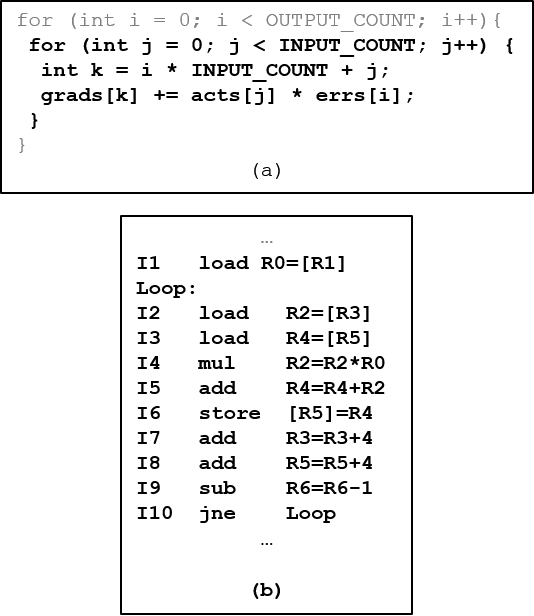
\includegraphics[width=2.4in]{Figures/gradient_code.png}
\caption{(a) Source code for computing gradients and (b) corresponding machine instructions of inner loop.}
\label{fig:gradient_code}
\end{figure}
\end{comment}
 